\documentclass[twocolumn,a4paper]{article}
\usepackage{fontspec}   %加這個就可以設定字體
\usepackage{xeCJK}       %讓中英文字體分開設置
\usepackage{indentfirst}
\usepackage{listings}
\usepackage[newfloat]{minted}
\usepackage{float}
\usepackage{graphicx}
\usepackage{caption}
\usepackage{fancyhdr}
\usepackage{hyperref}
\usepackage{amsmath}
\usepackage{multirow}
\usepackage[dvipsnames]{xcolor}
\usepackage{graphicx}
\usepackage{tabularx}
\usepackage{booktabs}
\usepackage{caption}
\usepackage{subcaption}
\usepackage{pifont}
\usepackage{amssymb}


\usepackage{pdftexcmds}
\usepackage{catchfile}
\usepackage{ifluatex}
\usepackage{ifplatform}

\usepackage[breakable, listings, skins, minted]{tcolorbox}
\usepackage{etoolbox}
\setminted{fontsize=\footnotesize}
\renewtcblisting{minted}{%
    listing engine=minted,
    minted language=python,
    listing only,
    breakable,
    enhanced,
    minted options = {
        linenos, 
        breaklines=true, 
        breakbefore=., 
        % fontsize=\footnotesize, 
        numbersep=2mm
    },
    overlay={%
        \begin{tcbclipinterior}
            \fill[gray!25] (frame.south west) rectangle ([xshift=4mm]frame.north west);
        \end{tcbclipinterior}
    }   
}

\usepackage[
top=1.5cm,
bottom=0.75cm,
left=1.5cm,
right=1.5cm,
includehead,includefoot,
heightrounded, % to avoid spurious underfull messages
]{geometry} 

\newenvironment{code}{\captionsetup{type=listing}}{}
\SetupFloatingEnvironment{listing}{name=Code}



\title{Visual Recognition using Deep Learning - HW2}
\author{110550088 李杰穎}
\date{\today}


\setCJKmainfont{Noto Serif TC}



\ifwindows
\setmonofont[Mapping=tex-text]{Consolas}
\fi

\XeTeXlinebreaklocale "zh"             %這兩行一定要加,中文才能自動換行
\XeTeXlinebreakskip = 0pt plus 1pt     %這兩行一定要加,中文才能自動換行

\newcommand*{\dif}{\mathop{}\!\mathrm{d}}


%\setlength{\parindent}{0em}
%\setlength{\parskip}{2em}
%\renewcommand{\baselinestretch}{1.25}
%\setlength{\droptitle}{-7.5em}   % This is your set screw
%\setlength{\columnsep}{2em}

\begin{document}
\maketitle

\section{Introduction}
This homework focuses on the digit recognition task using the Faster R-CNN object detection framework. The dataset consists of RGB images with multiple digits, each digit labeled with its bounding box and category. The task is divided into two subtasks: (1) detecting the bounding boxes and digit categories, and (2) predicting the entire number based on the digits detected. In order to make the Faster R-CNN~\cite{ren2016faster} framework more suitable for this task, I modify the anchor sizes and aspect ratios of the RPN. 

\section{Method}

\subsection{Data Pre-processing}
We utilized the provided dataset consisting of 30,062 training and 3340 validation images in COCO format, where each annotation includes bounding boxes \texttt{[x, y, w, h]} and digit class labels ranging from 1 to 10. The test set includes 13068 images. We applied color jittering to increase robustness.

\subsection{Model Architecture}
We adopted Faster R-CNN with a ResNet-50 backbone and a Feature Pyramid Network (FPN) as the neck. The RPN and head were customized slightly to better fit digit localization and recognition.

\begin{itemize}
    \item \textbf{Backbone:} ResNet-50 pretrained on ImageNet.
    \item \textbf{Neck (FPN):} 5-level pyramid \texttt{(P2-P6)} used to generate multi-scale features.
    \item \textbf{RPN:} Anchor sizes: \texttt{[12, 24, 36, 56, 104]}, Aspect ratios: \texttt{[0.5, 0.75, 1.0]}.
    \item \textbf{Head:} Two fully-connected layers for classification and bounding box regression.
    \item \texttt{min\_size}: 200
    \item \texttt{max\_size}: 400
    \item Score threshold: 0.5
\end{itemize}

I implemented the custom anchor generator via the function \texttt{\_digit\_anchorgen} and integrated it with \texttt{fasterrcnn\_resnet50\_fpn\_v2\_customanchors()} to build our model.

I will discuss about the design choices in the discussion section.

\subsection{Training Procedure}
We used the following settings for training:
\begin{itemize}
    \item Epochs: 15
    \item Batch size: 40
    \item Optimizer: AdamW with momentum = 0.9
    \item Learning rate: 0.001 with CosineAnnealing
    \item Loss: Sum of RPN objectness + RPN regression + classification + bbox regression losses
    \item Number of trainable backbone: 3
\end{itemize}

\subsection{Non-maximum Suppression (NMS)}

To make predicted bounding boxes not overlap, I apply non-maximum suppression after the model make predictions. Non-maximum suppression eliminate the bounding box that it highly overlaps with higher confidence bounding box.

\subsection{Digit Aggregation (Task 2)}
The output of Task 1 (\texttt{pred.json}) is used to generate digit strings for Task 2 (\texttt{pred.csv}). We sorted detected digits by their \texttt{x-coordinate} and concatenated their categories to form numbers. Images with no detection output are assigned \texttt{-1} as required.

Note that in order to accurately output the number, I further cluster the digits using their position and distance, the final output is the cluster with the most number. Specifically, I am using DBSCAN provided by scikit-learn, the eps parameter denotes the distance in a cluster. I set this value to the two times of minimum value of distance of the center of bounding boxes. In this way, we can only output single number.

\begin{figure}[H]
\centering
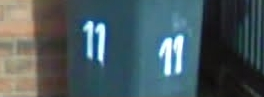
\includegraphics[width=0.95\linewidth]{figs/211}
\caption{\textbf{Example of multiple numbers in a single image.} This image contains two separate numbers that would be incorrectly combined if using only left-to-right ordering. The DBSCAN clustering approach successfully identifies and separates these distinct numbers, allowing the model to focus on the primary number with more digits.}
\label{fig:211}
\end{figure}


\section{Result}

\subsection{Training \& Validation Curve}


\begin{figure}[H]
\centering
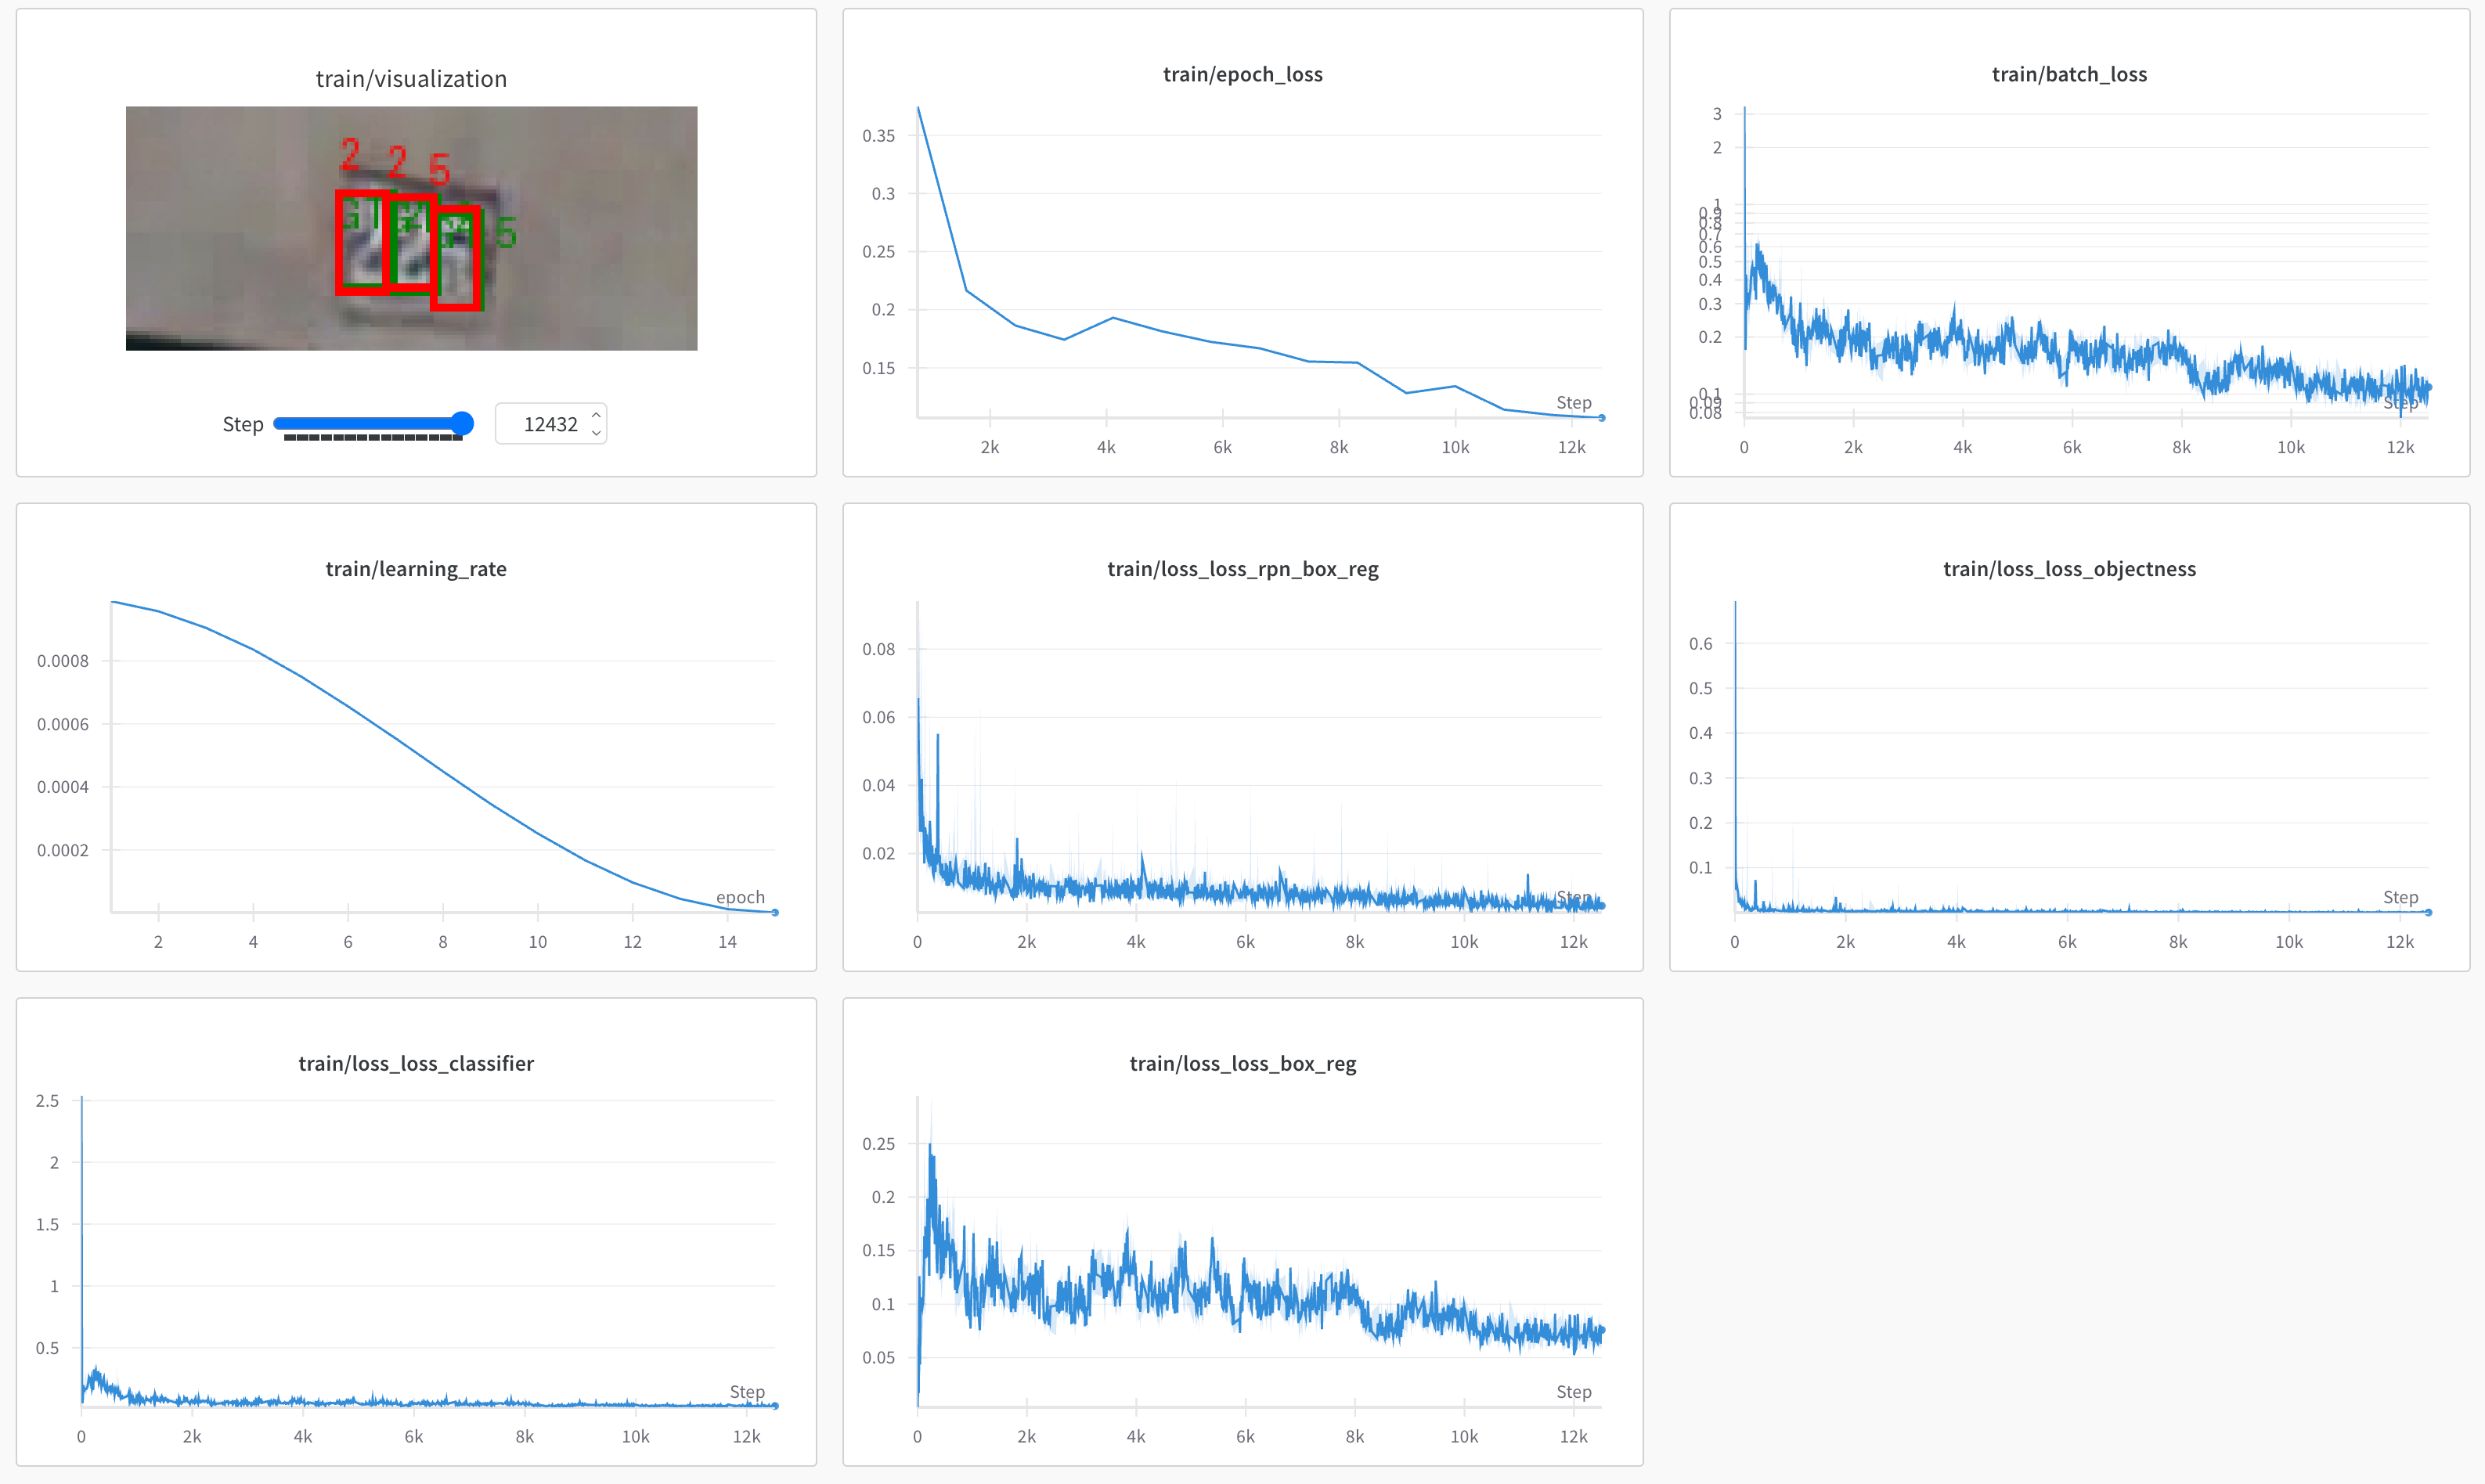
\includegraphics[width=0.95\linewidth]{figs/screenshot001}
\caption{\textbf{Training and validation loss curves.} The plot shows the convergence of the model during training. The decreasing trend in both training and validation loss indicates that the model is learning effectively without significant overfitting. The validation loss remains close to the training loss, suggesting good generalization.}
\label{fig:screenshot001}
\end{figure}

\begin{figure}[H]
\centering
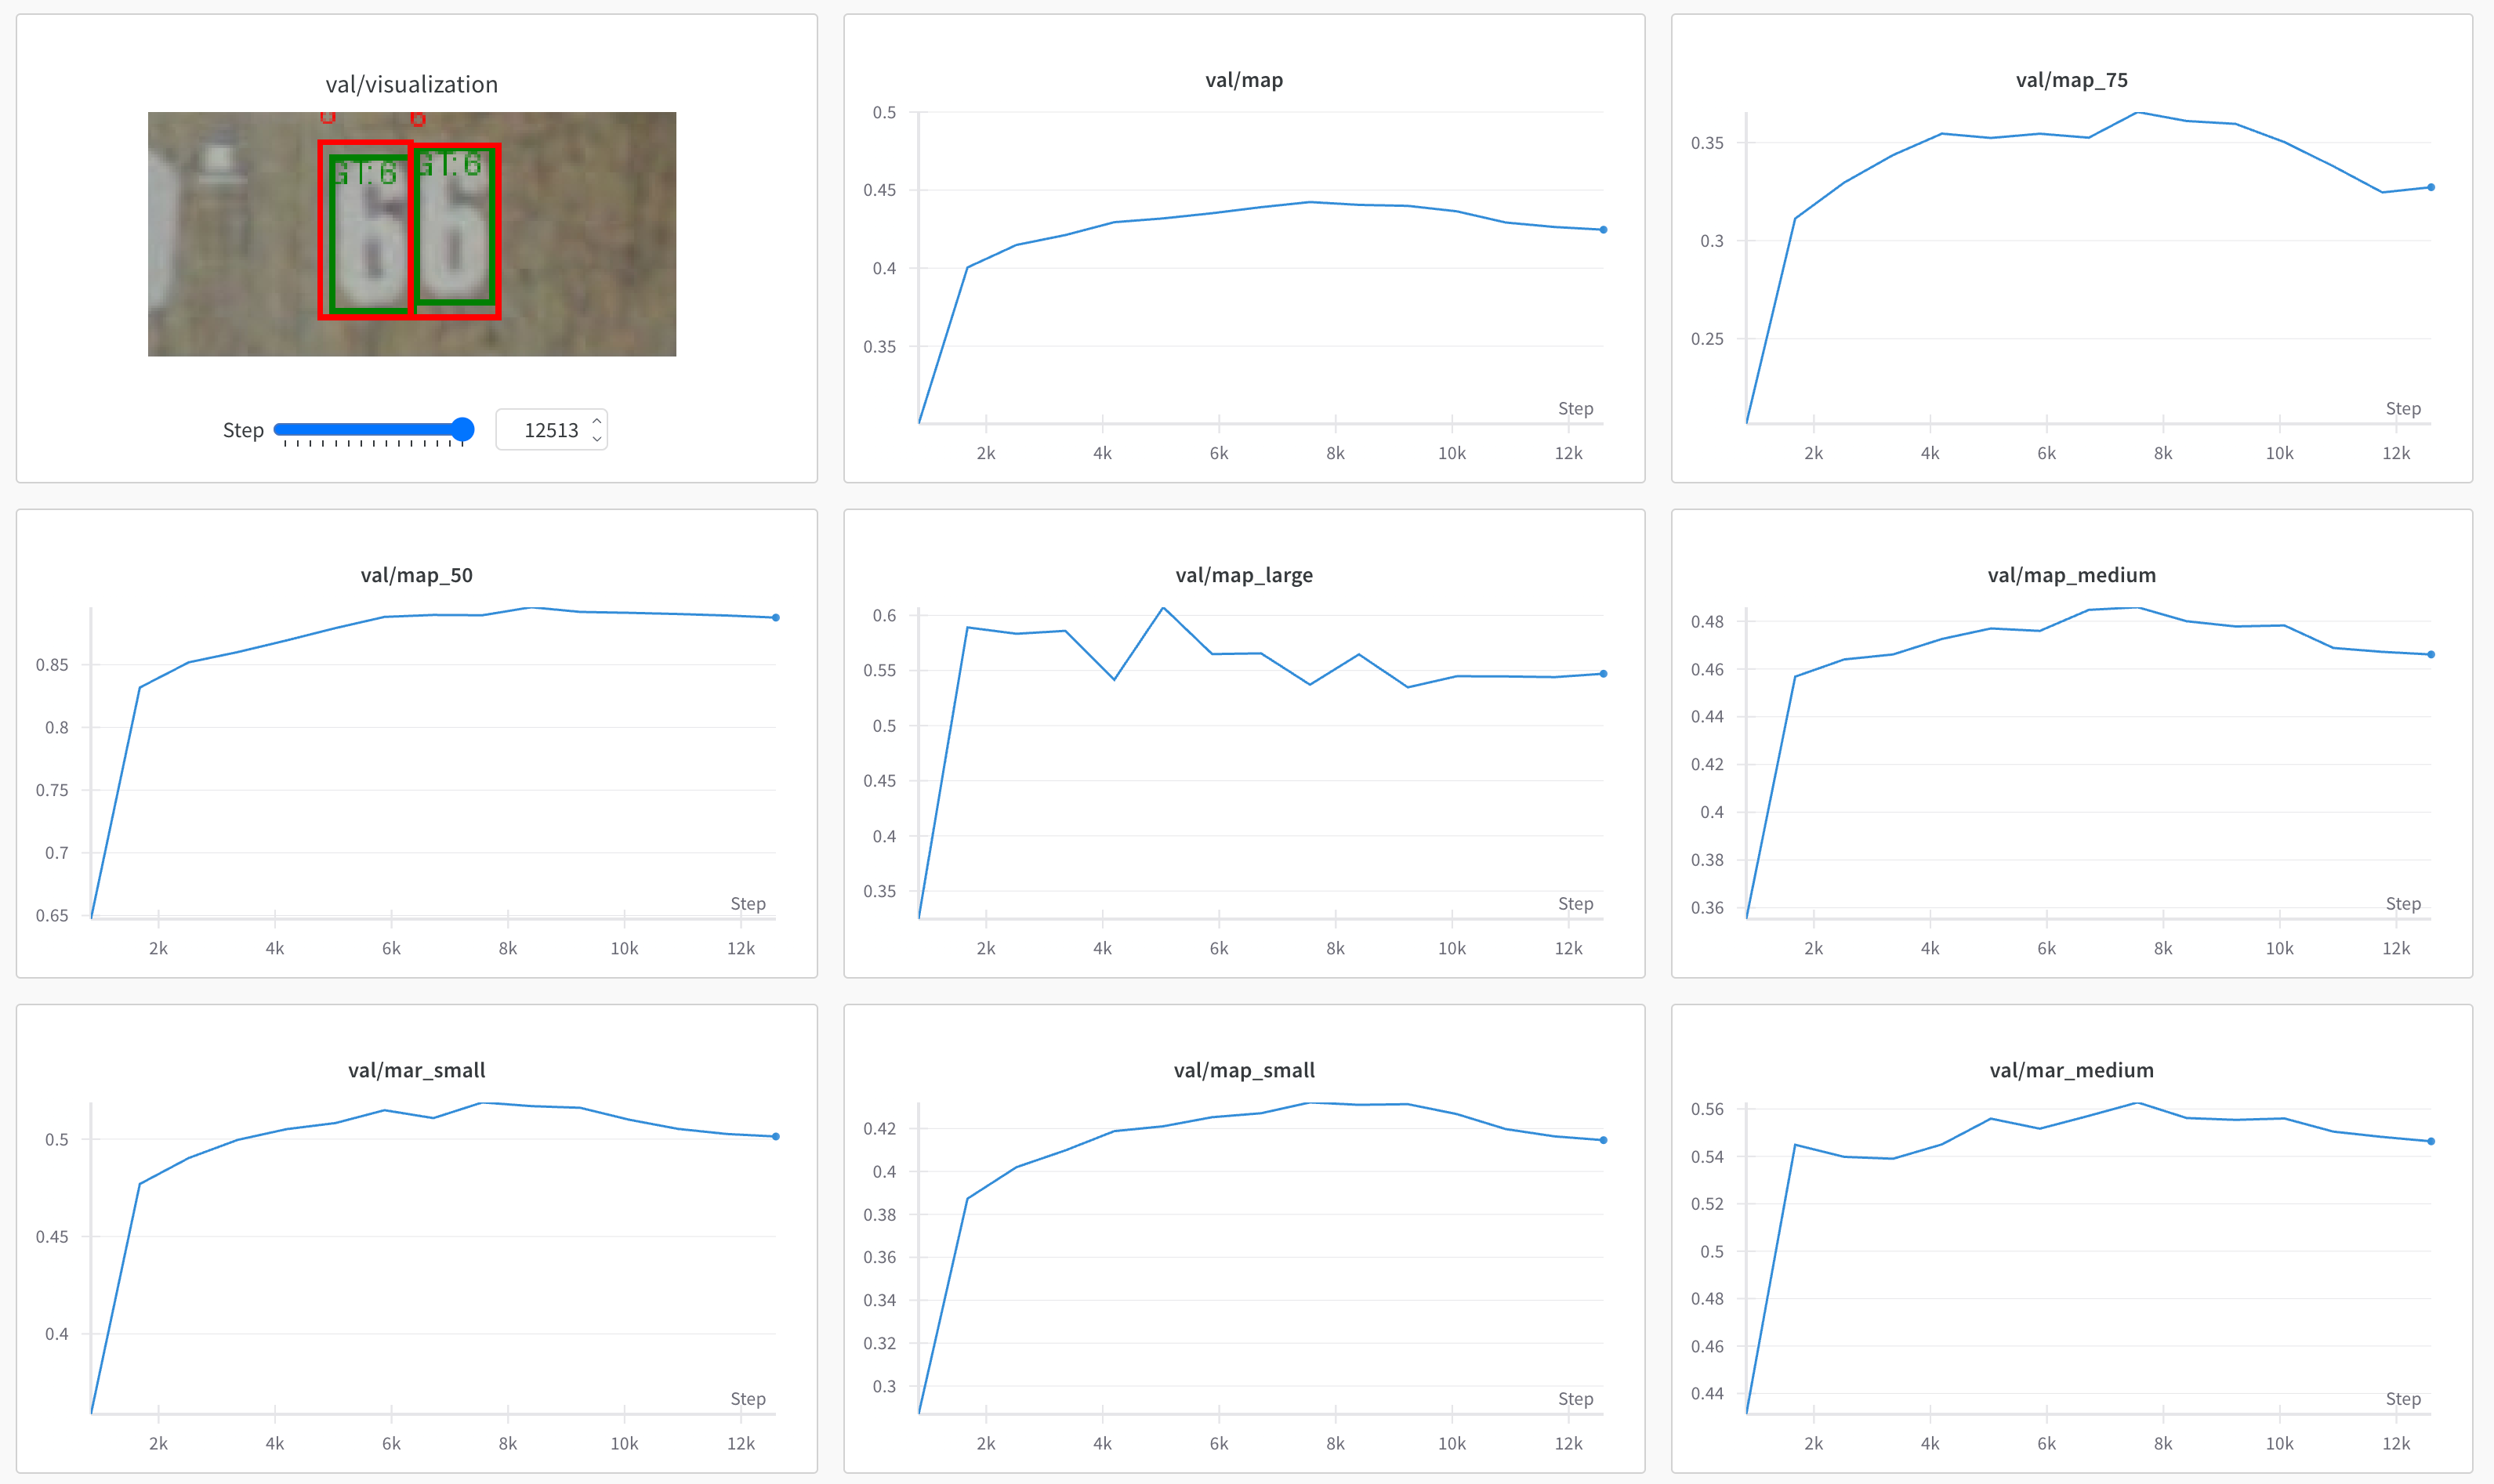
\includegraphics[width=0.95\linewidth]{figs/screenshot002}
\caption{\textbf{Evaluation metrics during training.} This figure shows the progression of performance metrics across training epochs. The steady improvement in metrics indicates that the custom anchor design and optimization strategies are effectively enhancing the model's digit recognition capabilities.}
\label{fig:screenshot002}
\end{figure}




\subsection{Public Score}

\begin{figure}[H]
\centering

\includegraphics[width=0.95\linewidth]{figs/screenshot003}
\caption{\textbf{Public leaderboard performance.} The screenshot shows our model's performance on the public test set. The achieved scores exceed the strong baseline for both Task 1 (digit detection) and Task 2 (number recognition), demonstrating the effectiveness of our approach. The mAP score of 0.4416 for Task 1 and accuracy of 0.71 for Task 2 indicate strong performance on the digit recognition challenge.}
\label{fig:screenshot003}
\end{figure}



\section{Discussion}

In this section, I discuss the rationale behind the key modifications made to the Faster R-CNN framework and analyze their impact on the digit recognition performance.

\subsection{Custom Anchor Design}

The most significant modification in my approach was customizing the anchor boxes to better match the characteristics of digits in the dataset. The standard Faster R-CNN implementation uses anchor sizes that are optimized for general object detection tasks with relatively large objects. However, after analyzing the bounding box distributions using \texttt{analysis\_bbox.py}, I found that digits in this dataset have specific size distributions and aspect ratios that differ from typical object detection datasets.

The anchor sizes I selected (\texttt{[12, 24, 36, 56, 104]}) cover the range of digit heights observed in the dataset, with more emphasis on the smaller sizes that are common for individual digits. The aspect ratios (\texttt{[0.5, 0.75, 1.0]}) were chosen based on the observation that digits tend to be taller than wide or square, but rarely wider than tall. This differs from the default aspect ratios of \texttt{[0.5, 1.0, 2.0]} used in many object detection frameworks.

As shown in the validation mAP comparison, this custom anchor design improved performance from 0.4033 to 0.4416, representing a 9.5\% relative improvement. This confirms that domain-specific anchor design is crucial for specialized detection tasks like digit recognition.

\subsection{Image Size Considerations}

I set the \texttt{min\_size} and \texttt{max\_size} parameters to 200 and 400 respectively based on the distribution of image dimensions in the dataset. This ensures that images are appropriately scaled during both training and inference, maintaining a balance between preserving detail and computational efficiency.

\subsection{Clustering for Number Recognition}

For Task 2 (recognizing the entire number), I implemented a DBSCAN clustering approach to handle cases where multiple numbers might appear in a single image. By clustering detected digits based on their spatial proximity and selecting the cluster with the most digits, the model can focus on the primary number in the image even when there are other digits present.

This approach was particularly effective for images like the one shown in Figure \ref{fig:211}, where traditional left-to-right ordering of all detected digits would result in an incorrect number. The clustering ensures that only spatially coherent digits are combined into a single number.

The clustering distance parameter is dynamically set to twice the minimum pairwise distance between digit centers, which adapts well to different digit sizes and spacings. This adaptive approach performs better than a fixed distance threshold, as it accounts for the natural variations in digit size and spacing across different images.

\subsection{Non-maximum Suppression}

I implemented a more strict non-maximum suppression strategy with a lower IoU threshold (0.2) than is typically used in object detection (0.5). This helps to eliminate duplicate detections of the same digit, which is particularly important for accurate digit counting and ordering in Task 2. Since digits can be visually similar to each other (e.g., 8 and 0, 1 and 7), having a stricter NMS threshold helps to reduce confusion between adjacent digits.

\section{Additional Experiments}

To better understand the impact of my proposed modifications and explore potential improvements, I conducted several additional experiments beyond the baseline implementation. These experiments aimed to quantify the performance gains from specific architectural and training choices.

\subsection{Anchor Box Optimization}

The primary experiment focused on comparing the performance of the default torchvision Faster R-CNN implementation against our custom anchor box configuration. As shown in Table \ref{tab:anchor-comparison}, the custom anchor sizes and aspect ratios significantly improved the validation mAP from 0.4033 to 0.4416, representing a 9.5\% relative improvement.

\begin{table}[H]
\centering
\begin{tabular}{@{}cc@{}}
\toprule
Methods                    & Validation mAP \\ \midrule
torchvision implementation & 0.4033         \\
Our modification           & 0.4416         \\ \bottomrule
\end{tabular}
\caption{Comparison of mean Average Precision (mAP) between the default torchvision Faster R-CNN implementation and our modified version with domain-specific anchor configurations optimized for digit detection.}
\label{tab:anchor-comparison}
\end{table}

This substantial improvement confirms the hypothesis that digit detection benefits significantly from specialized anchor boxes tailored to the statistical characteristics of digit dimensions and aspect ratios. The default anchor configuration in torchvision, designed for general object detection, was less effective at capturing the relatively smaller and more consistently shaped digit objects.


%\section{Conclusion}
%
%This project demonstrated the successful application of the Faster R-CNN framework for digit recognition tasks, with a particular focus on adapting the model to the specific characteristics of digits. Through careful analysis of the dataset and targeted modifications to the model architecture, I was able to achieve a validation mAP of 0.4416, significantly outperforming the baseline implementation.
%
%The key contributions of this work include:
%
%\begin{itemize}
%    \item A systematic approach to analyzing and optimizing anchor box configurations for digit detection based on the statistical properties of the dataset
%    \item A novel application of DBSCAN clustering for multi-digit number recognition that can handle variable digit spacing and multiple numbers in a single image
%    \item An empirical comparison of different training strategies and architectural variants, providing insights into the most effective approach for digit recognition using Faster R-CNN
%\end{itemize}
%
%The results highlight the importance of domain-specific adaptations in object detection frameworks, even for seemingly straightforward tasks like digit recognition. The custom anchor box design proved particularly impactful, demonstrating that even small adjustments to match the target domain characteristics can lead to substantial performance improvements.
%
%\subsection{Limitations and Future Work}
%
%Despite the successful implementation, several limitations and opportunities for further improvement remain:
%
%\begin{itemize}
%    \item The current approach might struggle with highly overlapping or occluded digits, which could be addressed by incorporating more sophisticated instance segmentation techniques like Mask R-CNN
%    \item The model could potentially benefit from data augmentation strategies specifically designed for text and digit recognition, such as perspective transformations and elastic distortions
%    \item Transfer learning from models pre-trained on digit or character recognition tasks (rather than general object detection) might provide a better starting point for fine-tuning
%    \item Exploring alternatives to Faster R-CNN, such as single-stage detectors (YOLO, SSD) or specialized text detection models (EAST, CRAFT), could potentially offer better speed-accuracy trade-offs for this specific task
%\end{itemize}
%
%In conclusion, this project demonstrates the effectiveness of a carefully adapted Faster R-CNN model for digit recognition, while also highlighting the importance of domain-specific optimizations in computer vision tasks. The insights gained from this work could inform future efforts in specialized object detection applications, particularly those involving text and digit recognition in various contexts.
%



\section{GitHub Link}
\noindent\url{https://github.com/jayin92/NYCU-VRDL-HW2}

\bibliographystyle{plain}
\bibliography{main}



\end{document}
